%
% File naaclhlt2010.tex
%
% Contact: nasmith@cs.cmu.edu

\documentclass[11pt,letterpaper]{article}
\usepackage{naaclhlt2010}
\usepackage{times}
\usepackage{latexsym}
\usepackage{graphicx}
\usepackage{apacite}
\usepackage{amsmath}

\setlength\titlebox{6.5cm}    % Expanding the titlebox

\title{Neural Networks for Predictive Ballistic Targeting}

\author{Vikram Chandrashekhar\\
  {\tt vchandr6@jhu.edu}
  \And
  Ran Liu \\
  {\tt rliu14@jhu.edu}}

\date{}

\begin{document}
\maketitle

\begin{abstract}
 We offer an algorithm for ballistic targeting which uses an online artificial neural network learner, and compare its targeting accuracy to existing ground truths, optimizing over certain parameters of the neural network. Ultimately we find we are able to achieve superior targeting accuracy across a wide set of data, but due to the non-convex nature of our network objective function, are unable to achieve the same maximum accuracy on certain datasets.
\end{abstract}

\section{Introduction and Background}

The task of ballistic targeting is such- given some input, e.g. the target's current position and velocity, one must choose a firing solution such that at some time in the future, the shot fired will intercept the target's future location. This problem is primarily important to game designers interested in improving the artificial intelligence (AI) of the turret.

There are many non-machine learning (i.e linear, circular targeting) and many machine learning methods (i.e neural nets, self-organizing maps, etc) to currently solve this task \cite{Guesgen_anartificial}. The current, "gold standard" for targeting methods are to compute trigonometric firing solutions using the velocity and position of the target. The two trigonometric firing solutions are linear and circular targeting; as the name implies, the linear targeting method assumes that the target will move at a constant velocity in a straight line. Similarly, the circular targeting method assumes the target is traveling in a circle of fixed radius.

The nature of the application of the problem is that the target can vary it's position very dramatically, especially when considering a human-controlled target. As such, it is important to use a method that is able to adapt to a changing underlying distribution of motion of the target. The limitation of the linear and circular models is that neither is able to adapt to changing types of motion since the underlying model (linear or circular motion) is fixed. Thus, we believe that an online machine learning algorithm is most suitable for the task. Since there may not necessarily be a linear relationship between the predictors and the output, and therefore, we require a method suitable for non linearly-separable data. The main advantage of an online algorithm is that it can adapt to changing underlying distributions of observed data and does not need to remain fixed in the case of the linear targeting \cite{Bottou98onlinelearning}.

We propose to use an artificial neural network to solve the targeting problem, as it is capable both of online learning and of classifying nonlinear data. The task at hand would be to implement a neural network algorithm that solves this task, and compare its performance against the baseline of existing non-machine learning targeting methods, e.g. linear, circular. The performance of these algorithms would then be measured using sets of targets with predefined movement patterns (linear, circular, composite), as well human-controlled targets.

The features used by the neural network will be position and velocity at each time step, including a variable time step history, to predict the future motion of a target. The position and velocity will be converted to coordinates relative to the location of the turret. The relative position and velocity will then be fed into the neural network. After creating a list of possible locations of the target that cover the range of all possible locations within the bullet travel time, the output of the neural network will be the best firing solution from the candidates.

\subsection{Problem Definition}
We conceptualize the ballistic targeting problem as such:
Two entities, a turret and target, exist in a two-dimensional Cartesian space. The turret has fixed position, and exists as a point, whereas the target is represented as a circle with fixed radius, and is able to move at speeds up to a limit fixed by the parameters of the model. At regular time intervals, the turret fires projectiles, which are also represented as points, are generated at the location of the turret, and have fixed speed, but can be set to move in any direction. Collisions between projectile and target occur when the position of the projectile is contained within the boundaries of the target circle and result in the destruction of the projectile. The targeting problem is to find the set of directions for the projectiles such that the number of resultant collisions is maximized.
\section{Methods}

\subsection{Software Overview}
In order to facilitate facile human control of targets as well as visualization of targeting algorithm results, we built a graphical user interface application, according to the model-view-controller software architecture pattern. The model portion of the application centers on the FieldModel class, which contains an object representation of the Cartesian space upon which turrets, targets, and projectiles exist. The Entity abstract superclass represents all entities which have the property of a position upon the Cartesian space, and the MoveableEntity abstract superclass represents all entities which have the properties of position and velocity. These positions are evaluated at discrete time intervals.

Turrets have TargetingAlgorithm objects bound to them, and at each firing invocation produce Projectile objects. The direction of these Projectile objects is determined by the TargetingAlgorithm which is bound to the Turret. Because targeting algorithms require access to the model state information in order to perform the necessary computations, we use the Observer design pattern/Java standard library interface, where the targeting algorithm is the observer, and the FieldModel is the observable. Therefore, whenever the state of the model is updated, all its observers are notified that an update has occurred, and the corresponding computations can be done for the next time-step. In our code, we include three implementations of TargetingAlgorithm: DirectTargeting, which commands that the turret should always fire at the current location of the target, LinearTargeting, which assumes that the target will always travel in straight lines with constant velocity, and returns FiringSolution objects accordingly, and NeuralNetworkTargeting, which reduces the ballistic targeting problem to a classification task, which is in turn handled by an artificial neural network learner. NeuralNetworkTargeting and its performance is the focus of this project.

We use the Java Swing graphical toolkit for the view portion of our application, along with the Observer pattern. The central class of the gui package, FieldView, is an Observer of the FieldModel. Therefore, when the model state is updated, the view is notified, and can be redrawn on the screen.
We have four types of controllers, one each for keyboard and mouse input, one that directly controls the FieldModel, and one that controls model playback, i.e. pauses and resumes playback. Additionally, if using target position data, rather than receiving input through the GUI, the playback controller controls the target position according to the file information. These controller objects process user input requests and invoke the appropriate methods upon model objects.

\subsection{Machine Learning Techniques}
% Explain the methods you will be using and why they are appropriate.
\subsubsection{Artificial Neural Networks}
Artificial Neural Networks (ANNs) are a set of models that are made up of many "layers" and "neurons". The "neurons" are represented by nodes in a given layer and the layers represent the sequential processing of input information as shown in Figure \ref{fig:NN}. The ANN is made up of an input layer, a series of hidden layers, and an output layer. In the case of a completely connected, feedforward ANN, all nodes in one layer are connected to all nodes in the subsequent layer. Since the targeting problem is such that all nodes require all the information from prior nodes, we implemented a fully connected, feedforward ANN with one hidden layer. We have chosen to use one hidden layer since we not only wanted to prevent overfitting from having too many parameters but also to allow the ANN to learn quickly as more layers dramatically increases the amount of time required to train the model.

\begin{figure}[h]
	\centering
	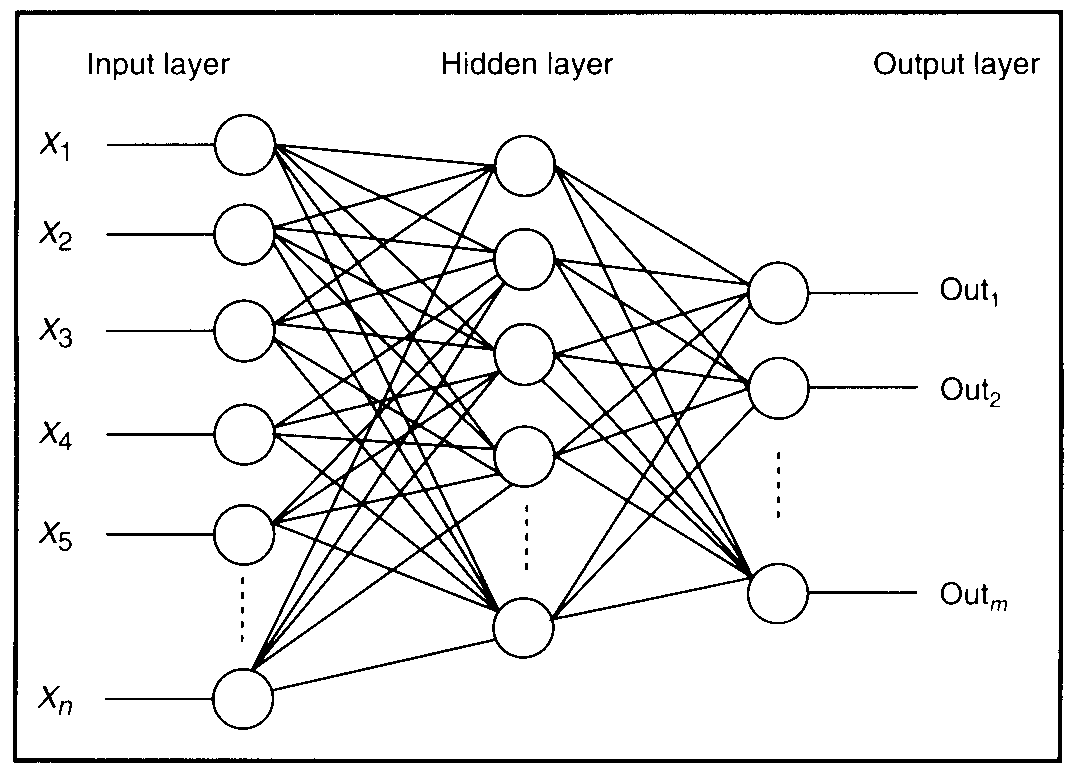
\includegraphics[scale = 0.8]{NN.png}
	\caption{Graphic representing ANN layers and nodes. }
	\label{fig:NN}
\end{figure}

\subsubsection{Forward Propagation}
In order to learn, the ANN has a set of weights connecting each node that must be optimized. Every connection from one node $i$ to another $j$ can be represented by a weight $w_{ji}^{(l)}$ where $l$ is the layer of the network and layer 1 is the input layer. The weights are initialized randomly to prevent any bias in the learned set of weights. In order to obtain outputs, the input set of features is propagated forward through the network as follows:
\begin{align} \label{eq:forward_prop}
a_k = \sum_{i = 1}^{D}{w_{ji}^{(1)}x_i}
\end{align}
where D is the number of input nodes, $x_i$ is the ith input node, and $a_k$ is the activation of node $k$ in layer 2. We use \eqref{eq:forward_prop} to determine the activations for each of the $k$ nodes in layer 2. We then perform a nonlinear transformation on the node activations using \eqref{eq:activation}. 
\begin{align} \label{eq:activation}
z_k = h(a_k)\\
h(a) = \frac{1}{1+\exp{(-a)}}
\end{align}
After applying the activation function \eqref{eq:activation} to each node, we repeat \eqref{eq:forward_prop} for layer 2 using the $z_k$ values in place of $x_i$.The output values obtained are then transformed again using the nonlinear activation function. The output values are scaled from 0 to 1 so that each node value represents a probability. These transformed values are now the $k$ predicted outputs from the ANN.

\subsubsection{Backpropagation}
In order to update the weights for each connection we attempt to minimize an error function. For this scenario, we chose to use a squared loss function \eqref{eq:error}.

\begin{align} \label{eq:error}
E = \frac{1}{2}\sum_k{y_k - t_k}^2
\end{align}
where $y_k$ is the value of output node $k$ and $t_k$ is the desired value for output node $k$. In order to update the weights to minimize the error, we take the derivative of the error function with respect to $w_{ji}$ as in \eqref{eq:er_grad}.
\begin{align} 
 \label{eq:er_grad}
\frac{dE}{dw_{ji}} = \delta_j{z_i}\\
\label{eq:delta1}
\delta_j = \delta_{j+1}h'(z_j)\\
\label{eq:delta}
\delta_{out} = h'(z_j)(y_k - t_k)
\end{align}

where $z_k$ is the value of node $k$ in a given layer after the nonlinear activation function has been applied to it. We store the outputs obtained from the ANN from forward propagation; once we obtain the "truth" or target values we would like each output node to have, we find the difference $\delta_{output}$ between our output value and the desired value using \eqref{eq:delta}. The values of $\delta$ are then backpropagated using \eqref{eq:delta1} to obtain the gradients for each weight. The weights are updated according to \eqref{eq:weight_update}.
\begin{align} 
\label{eq:weight_update}
w_{ji}^{t+1} = w_{ji}^{t} - \eta\frac{dE}{dw_{ji}}
\end{align}
where $\eta$ is a variable learning rate parameter.


\subsubsection{Feature Selection}
We began by choosing a set of features to provide as input to the ANN. The features that were selected are: relative velocity, and distance from turret. The relative velocity was obtained by calculating the change in relative position between two time ticks. Since the velocity is two-dimensional, the relative velocity represents two input features. This velocity is relative to the turret (i.e. the origin of the velocity vector is the center of the turret). The distance from the turret was calculated by subtracting the distances between the target in the current frame and the turret in the current frame. Therefore, we had a total of 3 input features into our system, representing 3 input nodes. In addition to these data from the current time step, we also decided to give the ANN a variable length history of target velocities and distances. The history was managed using a queue of fixed length; as more data was obtained by the ANN, the more recent features replaced the older features.

After obtaining all of the needed features, the features in the queue were concatenated and normalized so that the range of values of the features was 0 to 1. The purpose of the normalization was to warp the feature space so that it was a sphere rather than a potentially skewed ellipse (or any other shape). A spherical feature space is ideal as it allows gradient steps taken for each instance to be just as impactful as all other steps whereas for a skewed space, this may not be the case.

\subsubsection{Output Firing Solution}
The goal of our ANN is to determine the direction of the bullet that is most likely to hit the target. However, since our output from the ANN is a set of values corresponding to the number of nodes in the output layer, we must discretize the firing space. In order to do this, we calculate the range of valid directions by determining the bounds on the future location of the target and split the target space into $k$ solutions as in Figure \ref{fig:firing_soln}. Given the bounds, we varied the number, $k$, of outputs. Each of the output nodes represented one of $k$ possible firing solutions. After forward propagation through the ANN, the values of the output nodes are normalized to obtain probabilities of each firing solution. The solution with highest probability is chosen as the best firing solution.
\begin{figure}[h]
	\centering
	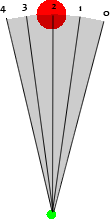
\includegraphics[scale = 0.8]{firing_arc_graphic.png}
	\caption{Graphic representing solution space and $k$ possible firing solutions.}
	\label{fig:firing_soln}
\end{figure}\\

\subsubsection{Online Learning}
In order for our ANN to be an online learner, it must receive a real-time input data stream. The data is provided as pre-generated or human test data which contains a list of turret and target positions. Using this data, at every time point, the ANN learner fires all $k$ output firing solutions; by keeping track of all the bullets, we continuously update the minimum distance to the target. We wait until the bullets are no longer physically able to hit the target, and then the use the minimum distance to target for each bullet as the "truth" value to compare to our estimation. Using these truth values, we update the ANN weights for each layer using backpropagation. Since bullets are fired at each time point, our ANN has a large amount of data to learn from.

\subsection{Experimental Methods}
We assess the accuracy of a targeting algorithms as the number of shots hit (number of projectiles which collide with targets) divided by the number of shots fired (number of projectiles created). While our GUI allows for model playback using live mouse control of target, all data collected was collected using generated or recorded target position data, so that all trials could be done using the same target position data. We used three generated data sets, and two recorded from mouse input. Additionally, while our software also allows for the same data to be run for multiple loops, while preserving targeting algorithm parameters between loops, we assess accuracy only for the first encounter of the learner with the data in question, as in real-world application, an online learner would need to be able to label data on its first encounter.

\section{Results/Discussion}

In situations where there is a consistent model that defines the distribution of data, online learning is not as effective as batch learning, as the online learner will have a period where it has not yet learned the parameters of the model. In the case of linear data, we see that the linear targeting algorithm clearly outperforms our online neural network. However, in cases where the linear model is not suitable, it achieves close to zero accuracy, whereas neural network targeting is still able to maintain some accuracy. One direct advantage that our online learner has over batch learners is that if we test on one dataset, and then another, whose data is labeled according to a different model, we are still able to maintain high quality predictions, whereas a batch learner would have had its parameters defined by the training data. The discrepancy in performance between linear and circular data can be explained in part by the methods used in feature selection- in circular data, relative velocity and distance remains constant, and thus, there is a consistent mapping between input and output labels for nearly the entire data set, whereas in linear data, distance and relative velocity are constantly changing.

The number of outputs with which we initialize our neural network targeter essentially is the resolution with which we compute firing solutions. At two outputs, the targeting algorithm can only choose between firing at the extreme left and right limits of the firing arc. While this simplifies the problem, it also often removes the correct firing solution from the output space. Therefore, we see an improvement in general in accuracy as we increase the number of outputs of the neural network. However, while we do not test extremely large numbers of output classes, it stands somewhat intuitively that there exists a point beyond which no benefit is gained by increasing the number of output classes. Because of the large number of weights which are introduced as parameters into our model, we introduce more possible local minima that our gradient descent method might move towards.
Increasing the memory of the neural network targeter increases the number of features which are input into the neural network. Because we restrict the number of hidden nodes, which forces the learner to produce a more simplistic representation of the input features, in theory the solution which our neural network produces neglects all non-important features. However, because we have a non-convex objective function, adding parameters merely complicates the energy landscape, and thus, there is a point at which we see decreased performance with more input features.
As with memory, we see that there is a happy medium for number of hidden nodes at which we see maximum performance. This follows intuitively for artificial neural networks in general, as when we have fewer hidden nodes than input nodes, we force a more efficient representation of the features in question. However, if there are many hidden nodes, we lose this capability.

Lastly, we choose a very high learning rate for our online neural network learner. This enables the learner to quickly adapt its parameters to the current distribution of data, and also implies that parameters learned from old data quickly decay as they are overwritten by new data. While this high learning rate often means that we overshoot the minimum with our gradient descent, the main benefit of using an online learner is in the ability to adapt to a changing distribution behind the data. Additionally, because of the way we frame the problem and define classification accuracy, higher accuracy is achieved if the learner is able to achieve some level of accuracy within a very small number of instances ? i.e. 15 or so instances, than if the learner is able to gradually converge closely to an optimal solution.

\section{Comparison to Proposal}
% What will appear in the final writeup.
Below is a bulleted list of what we achieved compared to our proposal:

\begin{itemize}
\item
We were successfully able to implement a neural network for the one target, one turret model (must achieve).
\item 
We were also able to test multiple configurations of the neural network but chose to use only a single hidden layer due to issues regarding overfitting and complexity of the problem (must achieve).
\item 
We created a GUI using Java and are able to visualize the motion of the target and the bullets of the turret in real time (expected to achieve).
\item 
We implemented the linear targeting algorithm but due to time constraints we were unable to implement the circular targeting method.
\end{itemize}


\bibliographystyle{apacite}
\bibliography{Final_Writeup}

\end{document}
